\subsection{Операторная схема схема замещения электрических цепей при нулевых и ненулевых начальных условиях}

Сущность операторного метода заключается в том, что функции вещественной переменной t, которую называют оригиналом, ставится в соответствие функция комплексной переменной p, которую называют изображением. В результате этого производные и интегралы от оригиналов заменяются алгебраическими функциями от соответствующих изображений (дифференцирование заменяется умножением на оператор р, а интегрирование – делением на него), что в свою очередь определяет переход от системы интегро-дифференциальных уравнений к системе алгебраических уравнений относительно изображений искомых переменных. При решении этих уравнений находятся изображения и далее путем обратного перехода – оригиналы.

Центральным принципом решения переходного процесса операторным методом является преборазования обычной электрической схемы к операторной схеме замещения переменной p. Полученную схему рассчитывают любым известным методом (методом узловых потенциалов, контурных токов или эквивалентных преобразований например).

На рисунках ниже приведена схема электрической цепи и её операторная схема замещения соответственно:

\begin{center}
  \begin{figure}[h!]	
    \center{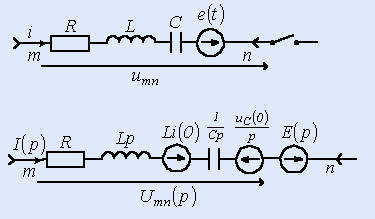
\includegraphics[scale=1]{replace_laplace.png}}
    \caption{Замещение}  
  \end{figure}
\end{center}

Таким образом правила преобразования основных элементов электрической цепи:

\begin{itemize}
\item Активное сопротивление остаётся без изменений
\item Конденсатор ёмкостью C заменяется двумя элементами — конденсатором 1/pC и источником ЭДС \item Uc(0)/p, который характеризует начальный заряд на конденсаторе
\item Индуктивность L заменяется двумя элементами — Индуктивностью pL и источником ЭДС L·iL(0), который характеризует начальный ток через индуктивность
\item Постоянный источник ЭДС или тока J, E заменяются на J/p и E/p соответственно
\end{itemize}

\pagebreak
